\chapter{Roadvet}
\label{cap:roadvet}
Este capítulo apresenta a contribuição principal deste trabalho, a aplicação RoadVet.

\section{Definição da Arquitetura do Sistema}

A arquitetura do sistema foi projetada segundo o modelo Cliente-Servidor, utilizando o padrão de \textit{APIs REST.} Essa abordagem justifica-se pelo fato de possibilitar o desacoplamento entre interface do usuário e regras de negócio, que no contexto do ambiente veterinário domiciliar é fundamental. Dessa maneira, o modelo Cliente-Servidor fornece uma independência ao cliente, de forma que os dados são processados localmente sem a necessidade da conexão com a internet. Assim quando a comunicação é reestabelecida com o servidor, a \textit{API REST} garante a comunicação entre ambos e salva os dados pendentes no banco de dados, conforme ilustrado na Figura~\ref{fig:arquitetura}.

%MODELAR A ARQUITETURA DO SISTEMA

\begin{figure}[H] 
    \centering 
    \caption{Diagrama de Arquitetura do Sistema} 
    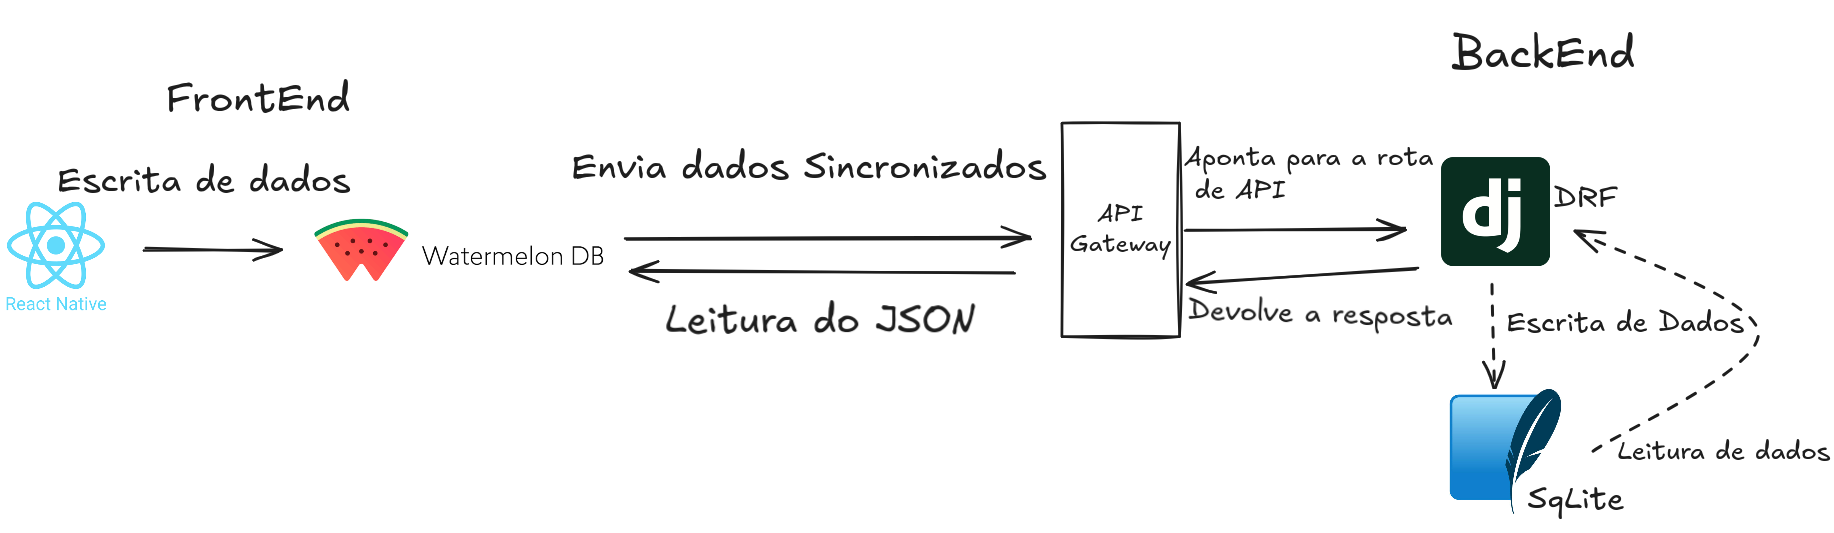
\includegraphics[width=\linewidth]{ArquiteturaSistema.png} 
    \label{fig:arquitetura} 
    \vskip 3pt
    \fonte{Elaboração própria}
\end{figure}


\section{Visão Geral}
% <<< REVISAR O TEXTO, POIS CITA QUE O APP TAMBÉM ATENDE PESSOAS SEM CRMV >>>
%EXPLICAR PARA QUEM É A APLICAÇÃO, MOSTRAR O FLUXO DETALHADO
%FAZER RELAÇÃO DAS TELAS COM OS REQUISITOS CITADOS
%NÃO DEIXAR IMAGENS UMA ABAIXO DA OUTRA SEM TEXTO
O RoadVet foi desde o princípio pensado com cuidado para atender os profissionais veterinários que se deslocam para atendimentos em regiões onde a rede mundial de computadores não funciona de forma devida, portanto a presente aplicação primordialmente atende à esses trabalhadores, de qualquer nível e que zelam pela saúde animal de forma autônoma, não impossibilitando que seja usado por profissionais de clínicas e estudantes em ambientes que possuem forte conexão com a internet, já que o aplicativo também opera normalmente com a presença de conexão, possibilitando o cadastro de pets, tutores e a criação de prontuários clínicos. No que tange a portabilidade do aplicativo, é importante destacar que ele foi pensado e desenvolvido para funciona especificamente em plataformas mobile, portanto não há a possibilidade de executá-lo em computadores de mesa ou notebooks.

\subsection{Fluxo Principal do Sistema}
Em relação ao fluxo do sistema e o primeiro contato do usuário com o RoadVet, o usuário é apresentado à tela de boas-vindas que consiste em dois botões: o primeiro destinado a cadastrar o novo usuário, redirecionando para uma tela de formulário de cadastro, o segundo para os usuários já cadastrados na plataforma, que redireciona para a tela de login. Esta tela é apresentada na Figura~\ref{fig:boasvindas}:

\begin{figure}[H] 
    \centering 
    \caption{Tela de Boas-Vindas do aplicativo} 
    \label{fig:boasvindas} 
    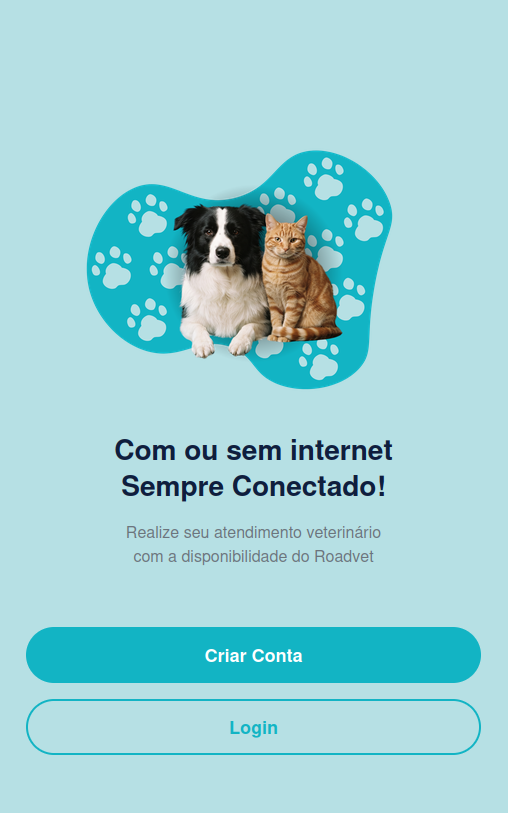
\includegraphics[
        width=0.5\linewidth,
        height=0.65\textheight,
        keepaspectratio
    ]{telaDeBoasVindasApp.png}
    \fonte{Elaboração própria.}
\end{figure}

Prosseguindo com esse fluxo, o usuário recém chegado irá clicar no botão de "Criar conta" e será redirecionado para o formulário aonde serão coletados seus dados pessoais, são eles nome completo, crmv, que é a licença que permite a prática formalizada da profissão do veterinário, email pessoal, telefone com DDD e senha, após isso o usuário será salvo no banco de dados do servidor. Segue a representação na figura ~\ref{fig:cadastro}:

\begin{figure}[H] 
    \centering 
    \caption{Tela de Cadastro do Aplicativo} 
    \label{fig:cadastro} 
    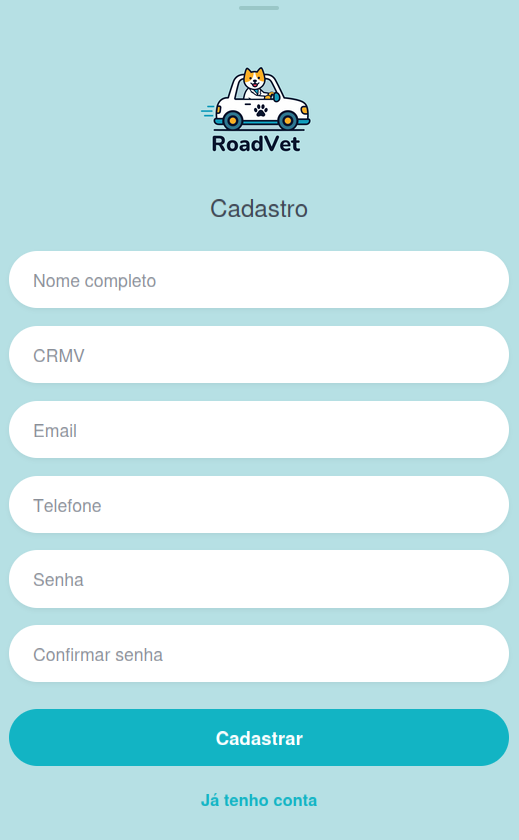
\includegraphics[width=0.5\linewidth]{teladDeCadastroApp.png}
    \fonte{Elaboração própria.}
    \vskip 3pt 
    \noindent{\small} 
\end{figure}

No caso de já existir um cadastro para o usuário, basta clicar no botão "Login", na tela de boas vindas, demonstrado na figura ~\ref{fig:boasvindas} e informar o email e senha para seguir os próximos passos, a tela de login está representada na figura ~\ref{fig:login}:

\begin{figure}[H] 
    \centering 
    \caption{Tela de Login do Aplicativo} 
    \label{fig:login} 
    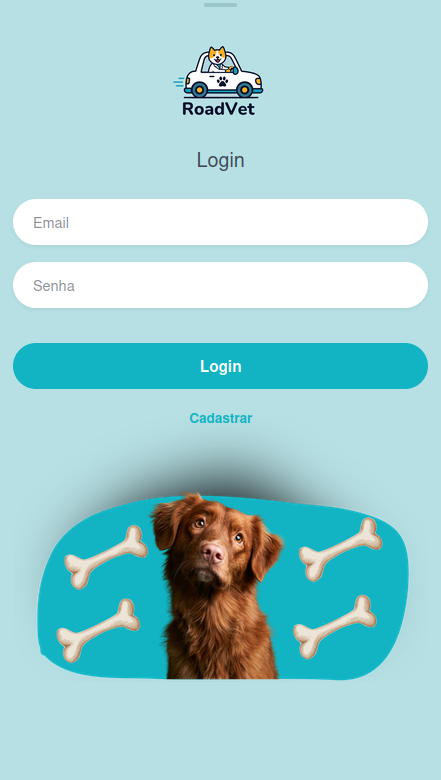
\includegraphics[width=0.5\linewidth]{telaDeLoginApp.png}
    \fonte{Elaboração própria.}
    \vskip 3pt 
    \noindent{\small} 
\end{figure}

Após a criação da conta, o veterinário será automaticamente direcionado para a tela principal do sistema, aonde o usuário é recebido com boas vindas no canto superior da tela, como também apresenta os ícones que descrevem que ele está com a conexão funcionando e o ícone de sair da conta, nessa ordem, os outros ícones redirecionam para a criação de um nova consulta, novo tutor, novo pet, lista de pacientes(pets), lista de tutores e o histórico de atendinentos, também nessa ordem. Logo abaixo está o painel de acompanhamento das últimas consultas feitas por ele, além da mensagem que reforça a sincronização com a internet. 

Nessa tela o usuário se depara com ícones na barra inferior da tela, o primeiro leva a tela atual, o segundo trata de todas as ações relativas aos pets, como criação, listagem e atualização, o terceiro trata das funcionalidades da entidade de tutores e o último é o ícone que leva à tela de prontuários e é nele que o usuário vai se redirecionar de acordo com o fluxo atual. Logo ao entrar nessa tela é possível pesquisar os prontuários existentes por nome, data e descrição, além da pesquisa é possível ordenar por cadastro mais recente, tutor ou pet em ordem alfabética e há a opção de filtrar canino, felino, com prescrição e sem prescrição. Todas as funcionalidades referentes aos prontuários estão disponíveis nessa tela, é possível criar um novo prontuário, ver a listagem deles, com nome do pet, data de criação e se é um cachorro ou gato, como também possui o ícone que mostrar se há ou não sincronização com o servidor. Segue uma representação fiel dessa tela na figura ~\ref{fig:painel}:

\begin{figure}[H] 
    \centering 
    \caption{Painel Principal do Aplicativo} 
    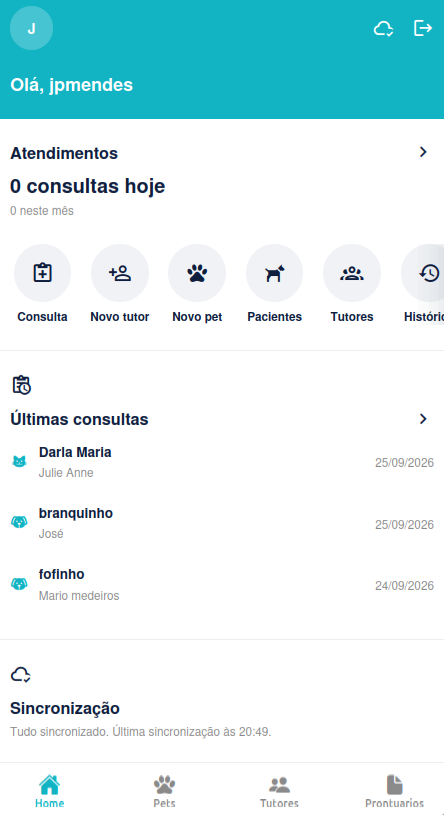
\includegraphics[width=0.5\linewidth]{painelPrincipalApp.png} 
    \fonte{Elaboração própria.}
    \label{fig:painel} 
    \vskip 3pt 
    \noindent{\small} 
\end{figure}

O próximo passo é clicar no quarto ícone  chamado "Prontuários", na parte inferior direita da tela, é nessa tela que acontece a orquestração dos prontuários, à primeira vista já é mostrada a listagem dos prontuários que já foram criados com o nome dos pets e data de criação, após essa ação o usuário é finalmente redirecionado para a tela de prontuários clínicos do aplicativo, representada na figura  ~\ref{fig:prontuarios}:

\begin{figure}[H] 
    \centering 
    \caption{Tela de Prontuários do Aplicativo} 
    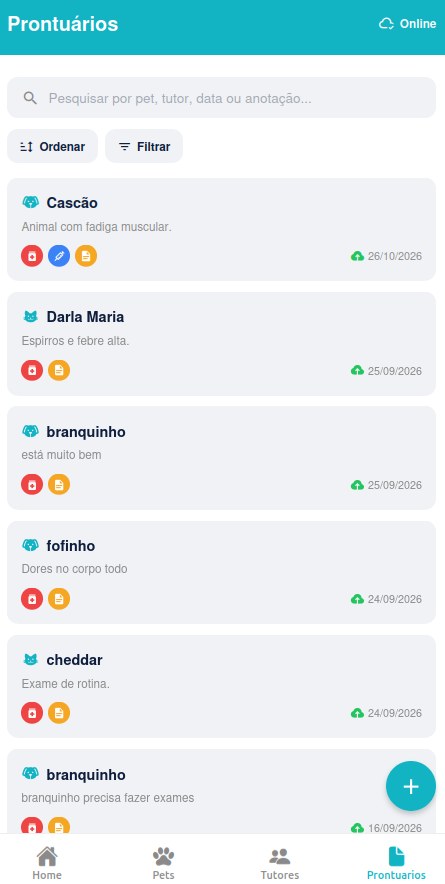
\includegraphics[width=0.5\linewidth]{telaDeProntuariosApp.png} 
    \fonte{Elaboração própria.}
    \label{fig:prontuarios} 
    \vskip 3pt 
    \noindent{\small} 
\end{figure}

Seguindo o fluxo que está sendo representado, a próxima ação é clicar no ícone de "+" no canto inferior direito da tela, depois disso o veterinário é finalmente levado a tela de criação do prontuário clínico, aonde são mostrados os pets que já estão cadastrados, com o nome de seu tutor ao lado. Além disso a tela conta com uma barra de pesquisas no canto superior, que permite filtrar os pets por nome, raça ou tutor relacionado. Abaixo dessa barra está representado o botão "+ Novo pet", responsável pela criação de um novo pet, caso seja o primeiro prontuário criado para ele, caso o pet já exista basta selecioná-lo na lista. A tela está representada na figura ~\ref{fig:criacaoprontuariolista}:

%\clearpage

\begin{figure}[H] 
    \centering 
    \caption{Tela de Criação de Prontuário} 
    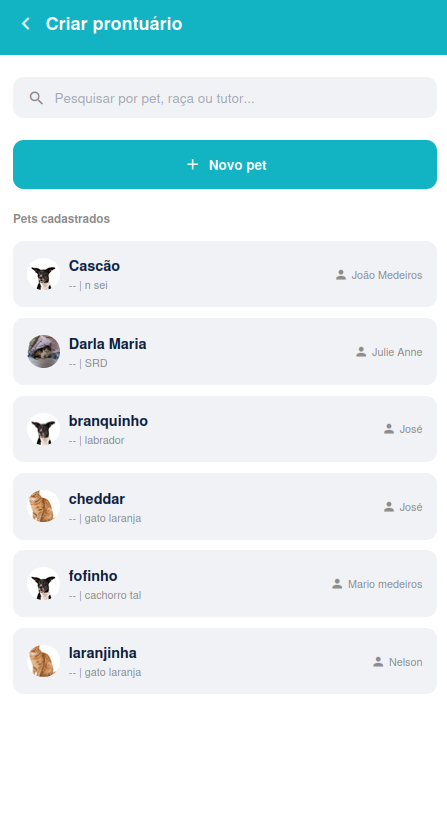
\includegraphics[width=0.5\linewidth]{TelaProntuarioCriacaoApp.png} 
    \fonte{Elaboração própria.}
    \label{fig:criacaoprontuariolista} 
    \vskip 3pt 
    \noindent{\small} 
\end{figure}

Após escolher uma entre as duas formas possíveis de criar o pet para o prontuário, o próximo passo é preencher o formulário de criação desse prontuário, devem ser fornecidos os seguintes dados em ordem: peso do animal em quilogramas, temperatura do animal em graus celsius, frequência cardíaca do animal, um texto referente a anamnese feita pelo veterinário, um texto para relatar o exame físico realizado, um texto com a prescrição após finalizar o exame e outros dados que serão informados na captura de tela seguinte, o que foi descrito está representado na figura ~\ref{fig:formularioprontuario1}:

%\clearpage

\begin{figure}[H] 
    \centering 
    \caption{Tela de Criação de Prontuário 1} 
    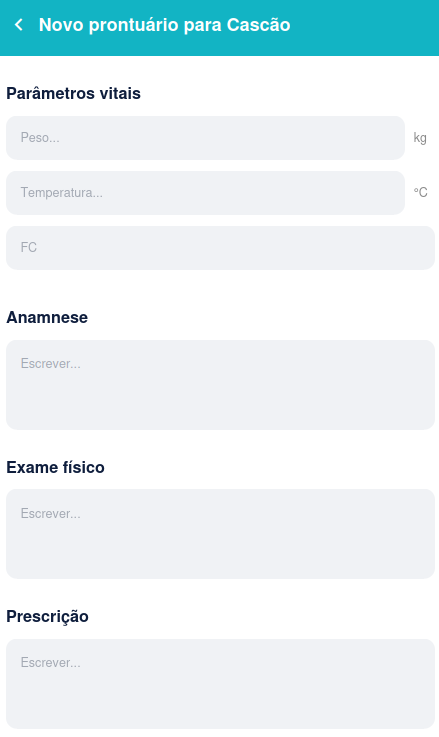
\includegraphics[width=0.5\linewidth]{TelaFormulario1.png} 
    \fonte{Elaboração própria.}
    \label{fig:formularioprontuario1} 
    \vskip 3pt 
    \noindent{\small} 
\end{figure}

Ainda no preenchimento do formulário, é preciso também inserir os dados de texto referentes a vacinas, solicitação de exames com anexo de PDF ou imagem e um texto contendo os resultados finais desse atendimento, também com anexo de PDF ou imagem e por fim salvar esse prontuário ou cancelar caso seja percebido algum erro. A tela está representada na figura ~\ref{fig:formularioprontuario2}:

%\clearpage

\begin{figure}[H] 
    \centering 
    \caption{Tela de Criação de Prontuário 2} 
    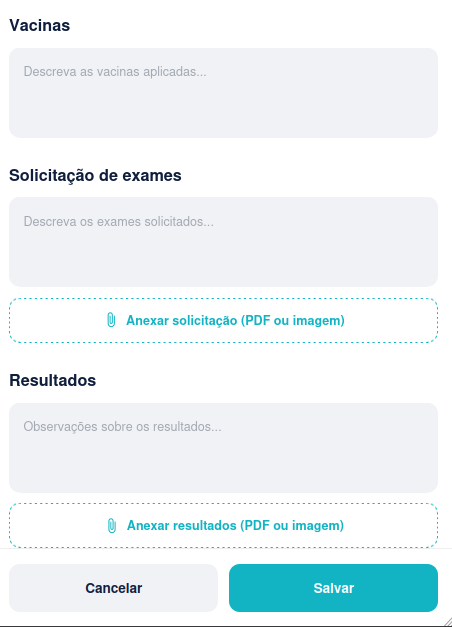
\includegraphics[width=0.5\linewidth]{FormularioProntuario2.png} 
    \fonte{Elaboração própria.}
    \label{fig:formularioprontuario2} 
    \vskip 3pt 
    \noindent{\small} 
\end{figure}

No caso do pet ainda não estar cadastrado no sistema, será necessário optar pela opção "Novo pet", logo abaixo da barra de pesquisa na tela, conforme foi apresentado na figura ~\ref{fig:criacaoprontuariolista}, serão preenchidas as informações para criar um novo pet, gato ou cachorro, deve-se fornecer imagem, o tutor responsável, caso já existam tutores cadastrados, nome, data de nascimento, peso em quilogramas, espécie e raça, depois basta clicar em "salvar" para cadastrar o animal ou "cancelar" caso haja algum erro. Segue na figura ~\ref{fig:criacaopet}, o que foi descrito agora.

%\clearpage

\begin{figure}[H] 
    \centering 
    \caption{Tela de Criação de Pet} 
    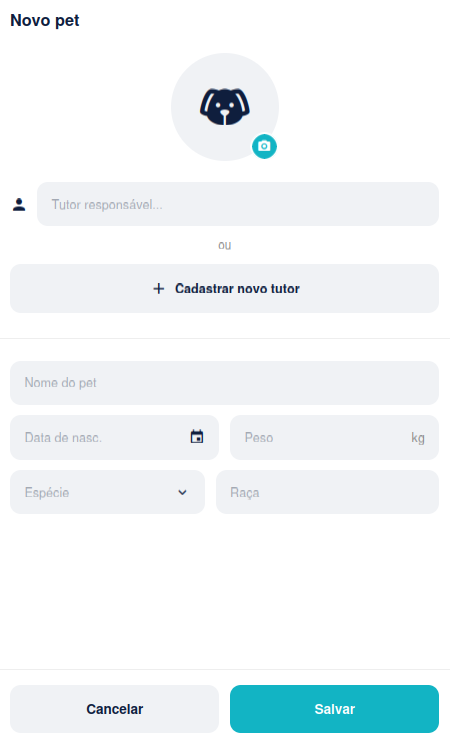
\includegraphics[width=0.5\linewidth]{NovoPetProntuario.png} 
    \fonte{Elaboração própria.}
    \label{fig:criacaopet} 
    \vskip 3pt 
    \noindent{\small} 
\end{figure}

No caso da não existência do tutor relacionado ao pet desejado, é possível clicar no botão "Cadastrar novo tutor", logo abaixo da opção "Tutor responsável", como mostrado na figura ~\ref{fig:criacaopet}, o usuário será redirecionado para a tela de cadastro do tutor, aonde serão fornecidos os dados de imagem, nome completo, cpf, data de nascimento, email, CEP, endereço, número, bairro, complemento, cidade, unidade federativa e dois telefones para contato. Isso é representado na figura ~\ref{fig:criacaotutor}

\clearpage

\begin{figure}[!htbp] 
    \centering 
    \caption{Tela de Criação do Tutor} 
    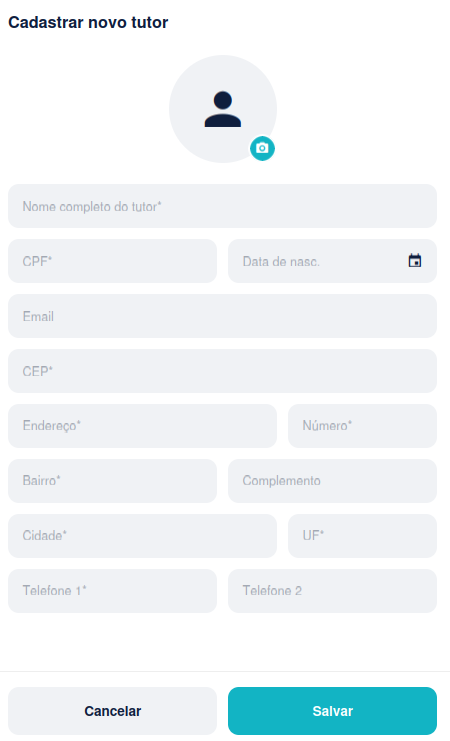
\includegraphics[width=0.5\linewidth]{CadastroTutorApp.png} 
    \fonte{Elaboração própria.}
    \label{fig:criacaotutor} 
    \vskip 3pt 
    \noindent{\small} 
\end{figure}

Se o passo a passo for seguido corretamente como descrito a cima, no final o usuário terá um prontuário profissional em seu aplicativo, totalmente funcional e aberto para edições e exclusão, em modo online e offline.

\section{Desenvolvimento do Aplicativo}
O desenvolvimento da aplicação foi executado fundamentando-se nos princípios e ensinamentos da Engenharia de Software, visando à construção de uma solução técnica plenamente funcional, modular e escalável. O sistema foi estruturado de forma desacoplada, dividindo-se entre a camada do cliente (\textit{front-end} móvel) e a camada de suporte (\textit{back-end}), permitindo a distribuição isolada das responsabilidades e a aplicação rigorosa das regras de negócio.

Como Ambiente de Desenvolvimento Integrado (\textit{Integrated Development Environment}, IDE) para ambas as vertentes do ecossistema, utilizou-se o \textit{Visual Studio Code} (\textit{VS Code}). O gerenciamento de configuração e o versionamento do código-fonte foram realizados por meio da ferramenta \textit{Git}, com o mapeamento sistemático dos incrementos em um repositório remoto hospedado na plataforma \textit{GitHub}. Essa abordagem garantiu a redundância do código-fonte entre a estação local de trabalho e o servidor remoto, servindo como um mecanismo de contingência para a recuperação de dados em caso de falhas de \textit{hardware}. Além disso houve a escolha do WatermelonDB como mecanismo de persistência local, garantindo assim o funcionamento do aplicativo somente na camada do cliente, em caso de perda de conexão. Reconhece-se que, para um ambiente de produção real e escalável no setor de saúde, a tecnologia chave-valor apresenta restrições de performance e segurança se comparada a bancos de dados relacionais locais como \textit{SQLite }ou documentais como \textit{Realm}.

No escopo da camada do cliente, a biblioteca \textit{React Native} foi adotada para o desenvolvimento da interface e da camada de apresentação do usuário. Nessa estrutura, implementou-se a lógica de persistência local utilizando a biblioteca \textit{AsyncStorage}, o que viabilizou a execução de operações fundamentais de criação, consulta, atualização e exclusão (\textit{Create, Read, Update and Delete}, CRUD) de prontuários clínicos diretamente no dispositivo móvel, mitigando os impactos decorrentes da falta de conectividade em campo.

Para a camada de suporte, utilizou-se o \textit{Django Rest Framework} (DRF) para a construção de uma API REST baseada na linguagem de programação \textit{Python}, enquanto o sistema gerenciador de banco de dados relacional \textit{SQLite} foi definido para a persistência e o armazenamento estruturado das informações. A lógica de negócio desenvolvida na retaguarda concentrou-se no gerenciamento da sincronização dos dados provenientes do cliente móvel. Desse modo, estabeleceu-se que, na presença de conexão ativa, as requisições são processadas e persistidas de forma imediata no banco de dados principal; em cenários de intermitência, o fluxo de dados aguarda a validação e as diretivas de sincronização disparadas pela camada superior da aplicação, mantendo a integridade das operações de criação, visualização, atualização e deleção.

\section{Estratégia de Persistência e Sincronização}
As estratégias utilizadas para persistir e sincronizar os dados em ambas as camadas projetadas no sistema foram estruturadas seguindo o conceito de arquitetura \textit{offline-first}. Essa abordagem garante que a aplicação móvel permaneça plenamente operacional para o médico veterinário mesmo em locais sem cobertura de rede, postergando a comunicação com o servidor para o momento em que a conectividade for restabelecida.

%REVISAR ESSE PARÁGRAFO
Na camada do cliente \textit{(front-end)}, o mecanismo de persistência local fundamenta-se na utilização da biblioteca \textit{WatermelonDB}. Por se tratar de um banco de dados reativo e local estruturado sobre o SQLite, a ferramenta permite gerenciar os dados relacionais dos prontuários clínicos diretamente no dispositivo de forma assíncrona. Para viabilizar o controle do fluxo de dados, cada registro manipulado localmente incorpora metadados de controle, especificamente uma marca temporal \textit{(timestamp)} da última modificação e uma flag indicadora de status de sincronização mapeada entre os estados pendente e sincronizado.

O processo de sincronização foi projetado a partir de uma estrutura de fila de eventos, cujo comportamento operacional é ditado pela detecção dinâmica do estado da rede, conforme descrito a seguir:

\begin{itemize}
    \item \textbf{Fluxo em Modo Offline:} Caso o dispositivo detecte a ausência de conexão à internet ou as requisições HTTP retornem falha por indisponibilidade de rede, as operações de CRUD são desviadas e executadas estritamente no \textit{WatermelonDB}. O registro correspondente é marcado com o \textit{status} de pendente e a operação é empilhada na fila local de sincronização.
    %REVER COMO FUNCIONA AGORA, CRIEI UMA ROTA ASYNC PARA A SINCRONIZAÇÃO
    \item \textbf{Fluxo em Modo Online e Reconexão:} Ao identificar o restabelecimento de uma conexão ativa e estável, a aplicação móvel inicia o esvaziamento da fila de maneira assíncrona. As operações pendentes são transmitidas sequencialmente à camada de suporte por meio de requisições HTTP utilizando os verbos adequados (\textit{POST} para criações, \textit{PUT} ou \textit{PATCH} para atualizações e \textit{DELETE} para exclusões), direcionadas aos respectivos \textit{endpoints} da API.
\end{itemize}

\begin{figure}[H] 
    \centering 
    \caption{Demonstração de Sincronização Bem-Sucedida no App} 
    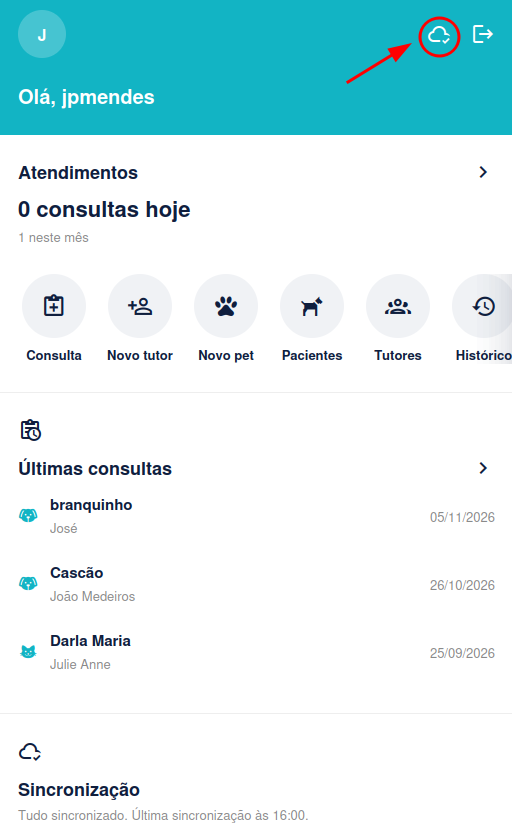
\includegraphics[width=0.5\linewidth]{sincronizacaoCap.png} 
    \fonte{Elaboração própria.}
    \label{fig:sincronizacaoCap} 
    \vskip 3pt 
    \noindent{\small} 
\end{figure}

Na camada de suporte (\textit{back-end}), o \textit{Django Rest Framework} (DRF) atua como o receptor e validador do lote de dados transmitidos pelo cliente móvel. Ao receber as requisições de sincronização, as rotas da API acionam as regras de negócio e os serializadores (\textit{serializers}) para garantir a integridade e consistência das informações antes de persisti-las de forma definitiva no banco de dados relacional \textit{SQLite}.

Para a resolução de potenciais conflitos de concorrência de dados, cenário comum em sistemas distribuídos e operados de forma desconectada, adotou-se a estratégia baseada na regra de que a última escrita é a que prevalece (\textit{Last-Write-Wins}, LWW). Através da comparação dos \textit{timestamps} enviados pelo dispositivo e os já existentes no banco de dados central, o servidor determina a versão mais recente do documento. Por fim, mediante o retorno bem-sucedido do servidor (códigos de \textit{status} HTTP 200 ou 201), o aplicativo atualiza o metadado do registro local no \textit{WatermelonDB} para o estado sincronizado e remove o item da fila de pendências, consolidando o ciclo de sincronização.
%REVISAR ESSA SEÇÃO, TALVEZ NÃO SEJA NECESSÁRIO CITAR O HTPP A ESSE NÍVEL
\section{Tecnologias para Desenvolvimento Mobile e Armazenamento Local}
\label{sec:fundamentacao-teorica-b}
Buscando o resultado de uma aplicação intuitiva e funcional, foram escolhidas as tecnologias React Native para a camada do cliente e o WatermelonDB para fazer a persistência dos dados nessa camada, de forma que os dados já sejam carregados no dispositivo do usuário de forma \textit{offline}. Para a persistência dos dados na camada do servidor foi utilizado o \textit{SQLite}, Sistema Gerenciador de Banco de Dados muito eficiente e leve. Já para a criação da Interface de Aplicação foi utilizado o\textit{ Django Rest framework}, que permite que os dados sejam enviados em formato de texto para a camada que se comunica com o usuário, garantindo a usabilidade total do sistema. Além dessas tecnologias de alto nível de desenvolvimento, o sistema em questão fez do uso do \footnote{\url{https://ics.uci.edu/~fielding/pubs/dissertation/top.htm}}Hyper Text TransferProtocol(HTTP) para o envio de textos entre a camada de suporte e a camda de cliente, como também a Arquitetura Rest para a criação da lógica de Interface de Aplicação de Informações com sua definitivas rotas.
